\chapter{Related work}
\label{chapter:related_work}

In this chapter we go through the related work in the field of deep learning, image classification
and image segmentation while describing various model architectures as well as recent
active learning approaches.

\section{Convolutional neural networks}
\label{sec:cnn_rw}

\subsection{First CNN}
\label{sec:cnn_rw:lecun}

The first convolutional neural network was proposed by LeCun et.
al. in late 1980s.~\cite{bib:lecun1989backpropagation}. Their approach has been
successfully applied to recognition of handwritten digits. Their dataset \cite{bib:lecun2010mnist}
consisted of roughly 9,298 images (later extended to 60,000 images),
which vary in sizes and styles. Image transformation
is applied to fit them to $16\times16$ pixel area, which prepares the images for feeding to the
network. The output consists of ten neurons, each one computing probability
of the given input being digit 0-9. The further development of this project was delayed
because of limited computational capabilities at that time.
Later, Matan et al.~\cite{bib:matan1992multi} extended this project to recognize
strings of digits because previous work was limited to only one-dimensional
input strings. Their approach includes recognizing 5-digit ZIP codes taken from
the U.S Mail using Viterbi module.
Since then, CNNs have been ignored by the computer vision community until the mid 2000s
because of lack of computational power.

\begin{figure}[h]
	\centerline{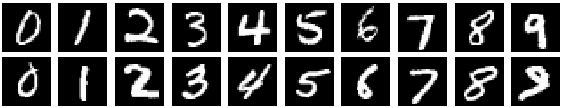
\includegraphics[width=0.6\textwidth]{images/mnist_example.png}}
	\caption[Example of digits from MNIST dataset]{Example of digits from MNIST dataset \cite{bib:lecun2010mnist}.}
	\label{img:mnist_example}
\end{figure}

\subsection{AlexNet}
\label{sec:cnn_rw:alexnet}

The great boom of deep neural networks has started after proposing
AlexNet~\cite{bib:krizhevsky2012imagenet}. Krizhevsky et al. competed in the
ImageNet Large Scale Visual Recognition Competition (ILSVRC) in 2012. ImageNet
\cite{bib:deng2009imagenet} is a dataset of over 15 million labeled high-resolution images
with around 22,000 categories. ILSVRC uses just a subset of them which is 1,000 categories.

AlexNet consists of 60 million parameters and 650,000 neurons. These neurons
are spread over five convolutional layers and 3 fully connected layers. The
last layer is 1000-way softmax, which produces the distribution over the 1,000 class
labels.
Convolutional layer filters are of sizes $11\times11$, $5\times5$ and $3\times3$.
Standard activation functions of neuron's input are \textit{tanh} or
\textit{sigmoid}. However, in terms of training time with gradient descent,
ReLU (rectified linear unit) activation function is
considered to be much faster. ConvNets with ReLU train several times faster.
To prevent model from overfitting, data augmentation and dropout methods are applied.

The full architecture is shown in Figure \ref{img:alexnet_architecture}.

\begin{figure}[h]
	\centerline{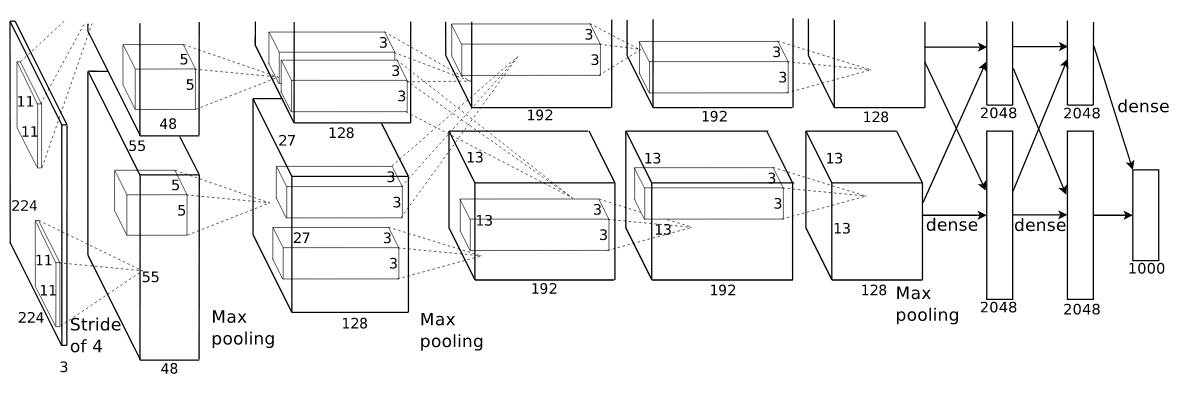
\includegraphics[width=0.9\textwidth]{images/alexnet_architecture.png}}
	\caption[AlexNet architecture]{AlexNet architecture. One GPU runs the
		top part while the other runs the bottom part. They communicate only at
		certain layers. (source \cite{bib:krizhevsky2012imagenet})}
	\label{img:alexnet_architecture}
\end{figure}

AlexNet outperforms previous feature-based methods lowering the error rate down by
40\% compared to hand-engineering approaches. On the test data, they achieve top-1 and
top-5 error rates of 37.5\% and 17.0\%.
Their success is based on using ReLU activation function, local response normalization,
dropout and stochastic gradient descent and in addition, usage of GPU during training
and testing process. The network became state-of-the-art in computer vision
classification.

\subsection{VGGNet}
\label{sec:cnn_rw:vggnet}

\textit{VGGNet} is an architecture proposed by Simonyan et al. \cite{bib:simonyan2014very}.
The idea is to use deeper networks with much smaller filters. The work contains models
which ranges from 16 to 19 layers and each one utilizes the smallest possible filters,
which is $3\times3$ in order to reduce number of parameters.
Some of the convolutional layers are followed by $2\times2$ max pooling layers with stride
2.
The stack of three $3\times3$ layers
has the same receptive field as one $7\times7$ layer and also fewer parameters
assuming that both input and output have $C$ channels, because
$3\cdot(3^2C^2) < 7^2C^2$. In addition, they incorporate three nonlinear functions
instead of one, which make the decision function more discriminative.
A downside of the VGGNet is that it uses a lot of memory due to expensive fully connected
layers. Most of the parameters are in the first fully connected layer, but it was found
that these FC layers can be completely removed with no significant performance downgrade
\cite{bib:szegedy2015going}.
Although the network's top-5 accuracy 92.7\% did not beat GoogLeNet (see subsection
\ref{sec:cnn_rw:googlenet}), it won the 1st prize in localization task in ILSVRC'14.

\subsection{GoogLeNet}
\label{sec:cnn_rw:googlenet}

GoogLeNet \cite{bib:szegedy2015going} won ILSVRC competition in 2014. It became the new
state-of-the-art CNN while achieving top-5 error rate of 6.67\%, which
is very close to human level performance.

\begin{figure}[h]
	\centerline{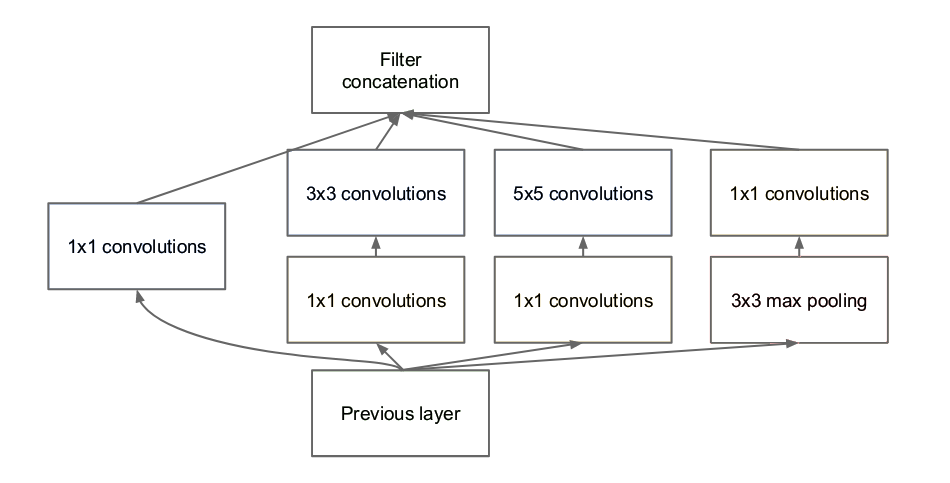
\includegraphics[width=0.8\textwidth]{images/googlenet_inception.png}}
	\caption[Inception module]{Inception module. (Image taken from \cite{bib:szegedy2015going})}
	\label{img:inception_module}
\end{figure}

Impressively, it consists of 22 layers, but the number of
parameters is reduced to just 4 million (compared to 7 layer AlexNet with 60 million
parameters). The main contribution this work has brought are \textit{Inception modules} which
are stacked on top of each other resulting in dramatic parameter reduction. Each one
contains independent convolution and pooling layers and their results are subsequently
concatenated into one output volume. Also, the
authors got rid of expensive fully connected layers.

The original naive inception module would be very computationally inefficient. Each
module would just increase the volume depth. Thus, the authors introduce an updated version
of the inception module (see Figure \ref{img:inception_module})
with $1\times1$ convolution put right before both $3\times3$ and
$5\times5$ convolutions and additionally after max pooling layer to reduce dimension.

\subsection{ResNet}
\label{sec:cnn_rw:resnet}

Looking at the popular architectures people started asking a simple question:
what happens if we continue stacking
deep layers on a plain CNN? Does it increase accuracy? The answer is no, as
He et al. describe and experimentally prove in \cite{bib:he2016deep}. Even though
deep models perform worse, it is not caused by overfitting.
They set a hypothesis
that this problem is an \textit{optimization problem}, and deeper models are harder to
optimize than more shallow networks. The reasoning behind this idea is that deeper networks
should perform at least as well as shallower ones (the solution is to copy
a shallow network and add identity layers on top).
The network won the 1st prize in 2015 on ILSVRC classification
task with $3.75\%$ top-5 error.
The network itself brings a ``revolution in depth'' since it is supposed to contain a
huge number of layers (it was 152 on ImageNet competition). The network features
special \textit{skip connections} and heavy use of \textit{batch normalization}.
The key idea is that instead of fitting $H(x)$ directly,
they rather use network layers to fit residuals $F(x) = H(x) - x$, which
is easier for the network to learn, see Figure \ref{img:residual_block}.
For deeper ResNet networks (50+ layers) they use so called bottleneck layers
(similarly to GoogleNet) in order to
improve efficiency. These layers contain additional $1\times1$ filters to decrease the
volume depth.

\begin{figure}[h]
	\centerline{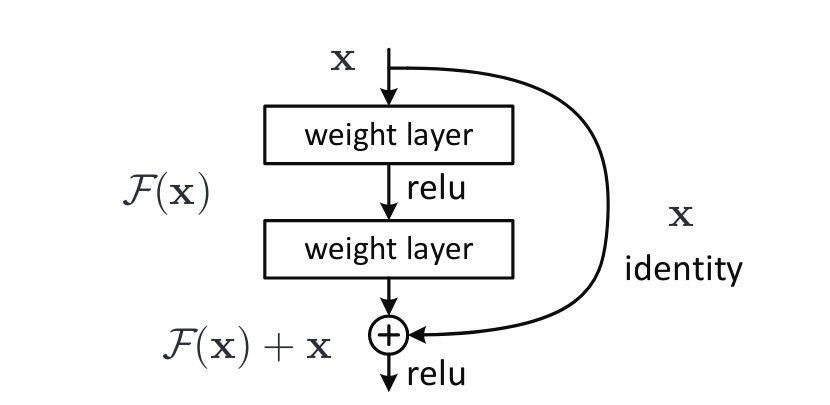
\includegraphics[width=0.6\textwidth]{images/residual_block.png}}
	\caption[Residual block]{Residual block. (Image taken from \cite{bib:he2016deep})}
	\label{img:residual_block}
\end{figure}

\section{Semantic segmentation using CNNs}
\label{sec:semantic_seg_cnn}

\subsection{Fully Convolutional Networks for Semantic Segmentation}
\label{sec:semantic_seg_cnn:fcn}

Fully convolutional neural networks proposed by Long et al. \cite{bib:long2015fully}
in 2014 popularized the use of end-to-end ConvNets for semantic segmentation of natural images.

They adapt contemporary classification networks like AlexNet, VGGnet, and GoogLeNet
and fine-tune them to segmentation task. The fully connected layers of these
classification networks are converted to fully convolutional layers
(see Figure \ref{img:transforming_fc_to_conv}).

\begin{figure}[h]
	\centerline{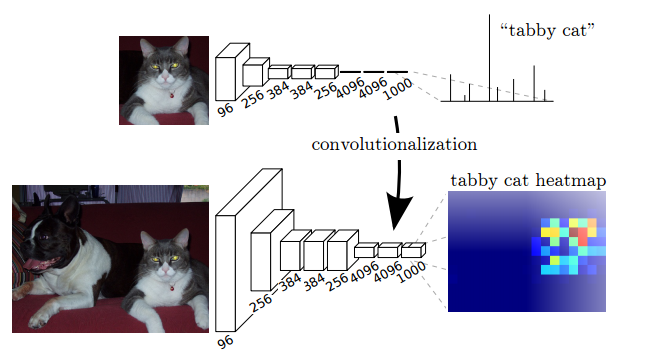
\includegraphics[width=0.9\textwidth]{images/transforming_fc_to_conv.png}}
	\caption[Transformation of fully connected layers into convolutions]{Transformation of fully connected layers into convolutions. (source \cite{bib:long2015fully})}
	\label{img:transforming_fc_to_conv}
\end{figure}

After convolutionalization, these layers produce class presence heatmaps in low resolution.
Some spatial information is lost because of pooling or strided convolutions,
so the mask must be upsampled at each stage using billinearly initialized deconvolutions.

They achieve state-of-the-art segmentation on PASCAL VOC dataset
\cite{bib:everingham2010pascal} with 20\% relative improvement to 62.2\% mean IU in 2012.

\subsection{U-Net}
\label{sec:semantic_seg_cnn:unet}

U-Net network \cite{bib:ronneberger2015u} got popular in biomedical image analysis.
Since the researchers in this area were forced to train the network with very little data,
image augmentation played a key role in this problem. The dataset the network is trained
on contains only 30 annotated images and outperforms the best methods on the ISBI challenge
for segmentation of neuronal structures in electron microscopic stacks. As discussed in
\cite{bib:ronneberger2015u}, it takes less than a second to segment image on a recent
GPU.

The architecture resembles the character "U", that is why it is called U-Net. On the left
side, there is encoder (or contracting path) which utilizes typical ConvNet architecture.
It contains $3\times3$ convolutions, followed by ReLU and max-pooling operations
for downsampling. Each layer in expanding path consists of upsampling of the feature map,
followed by $2\times2$ convolution, a concatenation of the feature map from the
contracting path and $3\times3$ convolution followed by ReLU. In terms of
data augmentation on microscopical images, they essentially just need
shift and rotation invariance as well as robustness to deformations and gray value
variation.

This network achieves 92\% mean IU on PhC-U373, beating the second best algorithm
with 83\%.

\subsection{SegNet}
\label{sec:semantic_seg_cnn:segnet}

SegNet~\cite{bib:badrinarayanan2017segnet} is another architecture of deep
convolutional neural networks for pixel-wise segmentation. The architecture
of encoder consists of 13 convolutional layers topologically
identical to first 13 layers of VGGnet~\cite{bib:simonyan2014very}.
The contribution of this work is mainly in the decoder, which uses pooling indices from the encoder
to perform upsampling, thus leaving high frequency details intact in the segmentation.
On the other side, neighboring information is missed when unpooling.
Therefore, the decoder does not have to learn upsampling and whole architecture
makes it more memory efficient.

\subsection{R-CNN, Fast R-CNN, Faster R-CNN, Mask R-CNN}
\label{sec:semantic_seg_cnn:maskrcnn}

Mask R-CNN published by He et al.~\cite{bib:he2017mask} in 2017 builds on previous
object detection works R-CNN~\cite{bib:girshick2014rich},
Fast R-CNN~\cite{bib:girshick2015fast} and Faster R-CNN~\cite{bib:ren2015faster}.

The original R-CNN is a four step process:
\begin{enumerate}
	\item Input an image
	\item Extract regions potentially containing objects (region proposals)
	\item Compute features from each region proposal using pre-trained CNN
	\item Classify each proposal using linear SVM
\end{enumerate}

The problem of R-CNN is that it is enormously slow. Also, the model does not learn to
localize objects using deep CNN. The contribution of Fast R-CNN is region of
interest (ROI) pooling module, which essentially extracts fixed-size window
from feature map. The network became end-to-end trainable but the performance
is dependent on selective search and therefore suffers at prediction time.

To make it even faster, Ren et al. proposed Faster R-CNN. It utilizes a so called
Region Proposal Network (RPN), which alleviates the need for selective search. Regions
of interests are generated and top $N$ are kept according to their objectness
score. In the original paper $N$ is set to 2,000.
Faster R-CNN architecture is capable of running at 7-10 FPS, which is a huge step towards
real-time object detection with deep networks.

Mask R-CNN has been published with two major contributions:
\begin{enumerate}
	\item Replaced ROI pooling module with more accurate ROI align module
	\item Inserted an additional branch out of the ROI align module to produce 
	mask of the object
\end{enumerate}

The network is therefore able to produce three outputs - bounding box of the object,
its mask and label.

\subsection{MultiNet}
\label{sec:semantic_seg_cnn:multinet}

In 2016, Teichmann et al. \cite{bib:teichmann2018multinet} published an interesting
work on road segmentation. In their approach they efficiently perform
classification, detection and semantic segmentation simultaneously.

Model architecture is traditional encoder-decoder. The difference is that there
is just one encoder producing rich features shared among all the tasks. These features
are then utilized by task specific decoders.
Encoder's weights are pre-trained on ImageNet classification data. They perform
experiments on VGG16 and ResNet architectures. The first one is called VGG-pool5
as it discards all fully-connected layers from VGG and pool5 is the last layer.
The second implementation is called VGG-fc7 because it only discards the final softmax
layer. Layers fc6 and fc7 are replaced by $1\times1$ convolutions. This allows the
network to process images of arbitrary size. For ResNet they implement 50 and 101
layer version of the network and discard fully-connected softmax.

Decoder architecture follows the FCN architecture \cite{bib:long2015fully}.
Segmentation is applied to input
downsampled by encoder to size $39\times12$ using $1\times1$ convolution layer. Then,
it is upsampled using three transposed convolution layers.

MultiNet's training strategy is fine-tuning. The encoder is trained to perform
classification on ILSVRC2012 dataset. But in practice, this step is omitted and
encoder is initialized using pre-trained weights of the respective networks they are using.
The second step is dedicated to replacing fully connected layers with
convolutional ones.

Authors evaluate the proposed model on KITTI dataset \cite{bib:Geiger2012CVPR},
which contains images
from various street situations captured from a moving platform in the city.
The segmentation module reaches MaxF1 score of 94.88\% with average precision of
93.71\% beating all other submissions. Moreover, the speed of prediction is 42.48ms on GPU
for all tasks, which is very efficient for real-time predictions.

According to their comparison of VGG and ResNet they observed that both ResNets
outperform VGGs, but noticed that there is a trade-off because VGGs are faster.

\section{Mobile models}
\label{sec:mobile_models_related}

Most of the work on semantic segmentation has focused on increasing accuracy of proposed
models with little attention to computational efficiency. While these networks have brought
state-of-the-art results, they often lack real-time prediction ability on devices with
limited computational power.

\subsection{MobileNets}
\label{sec:mobile_models:mobilenet}

Probably one of the most popular networks designed specifically for small devices in terms of
speed and computational power are \textbf{MobileNets} \cite{bib:howard2017mobilenets}.
These models come with two hyper-parameters, namely $\alpha$ and $\rho$. The former, also
called \textit{width multiplier}, is responsible for adjusting number of channels and
thins the network uniformly at each layer. For a given layer and multiplier $\alpha$,
the number of input channels becomes $\alpha M$ and the number of output channels
$\alpha N$, where $M$ and $N$ are original numbers. $\rho$, called 
\textit{resolution multiplier},
is applied to input image reducing size of input as well as internal representation
of subsequent layers. The architecture is composed of $3\times 3$
depthwise-separable convolutions except the first layer which is full convolution.
Authors test several variations of hyper-parameters and compare results on ImageNet dataset
and get $70.6\%$ top-1 accuracy.
Interestingly, MobileNet with $\alpha=1$ is almost as accurate as VGG16, while
being 32 times smaller and 25 times less compute intensive.

\vspace{5mm}
Sandler et al. \cite{bib:sandler2018mobilenetv2} continue in the work of searching for
efficient mobile models. Their architecture expands on aforementioned MobileNet and
they call it \textbf{MobileNetV2}. Each bottleneck stage consists of several bottleneck
layers, where the first one downsamples the representation with
$\textrm{stride}=2$ (with the exception in some stages). The rest of the layers in stage
utilize residual connection from input which is summed with output of the
pointwise convolution. Similarly to original MobileNet, it makes use of depthwise-separable
convolution which is preceded by $1\times 1$ convolution as shown in Figure
\ref{img:mobilenet_bottlenecks}. The model with $\alpha=1$ reaches
$72.0\%$ top-1 accuracy beating original MobileNet and reducing the number of parameters, as well
as the inference time. With $\alpha=1.4$ they get $74.7\%$ accuracy at the cost of
doubling the inference time.

Authors also compare semantic segmetation abilities of MobileNet and MobileNetV2 as
feature extractors on PASCAL VOC dataset. Encoders are followed by \textit{DeepLabV3}
decoder \cite{bib:chen2017rethinking} with various modifications. Benchmarks show that
their performance is almost equal but MobileNetV2 achieves it with fewer parameters.

\begin{figure}[h]
	\begin{center}
	    \subfloat[MobileNet bottleneck]{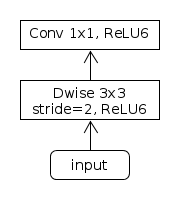
\includegraphics[width=0.33\textwidth]{images/mobilenet_bottleneck.png}}
		\quad
		\subfloat[MobileNetV2 bottlenecks]{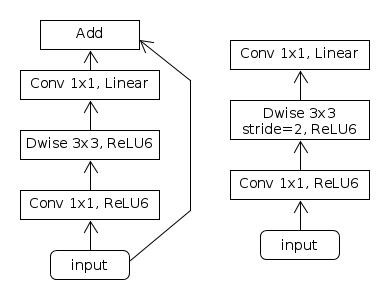
\includegraphics[width=0.48\textwidth]{images/mobilenetv2_bottleneck.png}}
	\end{center}
	\caption[Comparison of MobileNet and MobileNetV2 bottlenecks]{Comparison of MobileNet and MobileNetV2 bottlenecks.}
	\label{img:mobilenet_bottlenecks}
\end{figure}

\vspace{5mm}
The new generation of MobileNet is presented in the work of Howard et al.
\cite{bib:howard2019searching}. \textbf{MobileNetV3} is based on MobilenetV2 and MnasNet
\cite{bib:tan2019mnasnet} building blocks.
Automated platform-aware search NAS is used to look for global
network structures by optimizing each network layer and applies NetAdapt algorithm afterwards
to find out the number of filters per layer. Authors observe that some of the earlier
and final layers are more expensive than others, so they redesign and further optimize
them. Second half of bottleneck layers use newly proposed \textit{h-swish} nonlinearity,
since original swish ($\textrm{swish}(x) = x\cdot \sigma(x)$) includes computation of
sigmoid which is much more expensive in mobile environments.
Therefore, sigmoid has been replaced by its piece-wise linear hard analog and the h-swish 
function is defined as $\textrm{hswish}(x) = x\frac{\textrm{ReLU6(x+3)}}{6}$.
The final model comes in two versions, namely \textit{MobileNetV3-Large} and 
\textit{MobileNetV3-Small}, which are targeted to high and low resource use cases respectively.
The former reaches $75.7\%$ top-1 accuracy and the latter $67.4\%$, while being much more
efficient. The authors employ the models in semantic segmentation task and propose
\textit{Lite R-ASPP} segmentation head which is based on R-ASPP head that was proposed
by Sandler et al. \cite{bib:sandler2018mobilenetv2}. Experiments
are conducted on Cityscapes dataset \cite{bib:cordts2016cityscapes} and results
reported in mean IoU metric. MobileNetV3-Large attains similar performance as MobileNetV2
while being faster and MobileNetV3-Small performs similarly to MobileNetV2-0.5.

\subsection{ShuffleNets}
\label{sec:mobile_models:shufflenet}

Another family of light-weight convolutional network models is called \textbf{ShuffleNet}.
Zhang et al. \cite{bib:zhang2018shufflenet} propose the first model of this family.
The architecture makes use of \textit{pointwise group convolutions} and new idea
called \textit{channel shuffling}. The former has been introduced in
\cite{bib:krizhevsky2012imagenet} for distributing the model over two GPUs. If we stacked
two group convolutions on top of each other, the output channels would gain information
only from small fraction of previous channels. To address this, authors incorporate
channel shuffling, which divides previous groups into subgroups and then feeds each group
in next layer with different subgroup. Network's architecture starts with full $3\times 3$
convolution followed by max pooling and three stages with different numbers of shufflenet units
where the first one is used for spatial downsampling. Their experiments show that
channel shuffle increases accuracy and ShuffleNet with $\alpha=1$ (width multiplier) and
$\textrm{group}=8$ reached $67.6\%$ top-1 accuracy. With $\alpha=2$ they beat MobileNet
by $3.1\%$ while keeping the inference time.

Building upon ShuffleNet, Gamal et al. \cite{bib:gamal2018shuffleseg} experiment in the field
of semantic segmentation. Their network, called \textbf{ShuffleSeg}, employs ShuffleNet as
encoder. Experiments are conducted on Cityscapes dataset
and compare decoders U-Net, SkipNet, Dilation Frontend 8s and Dilation 4s. Results indicate
that SkipNet pretrained on coarse annotations with more labeled images beats other decoders
and provides a good trade-off between accuracy and real-time prediction. It is reported
to be capable of running at $15.7$ FPS on Jetson TX2.
\cite{bib:gamal2018shuffleseg, bib:Siam_2018_CVPR_Workshops}

\begin{figure}[!h]
	\centerline{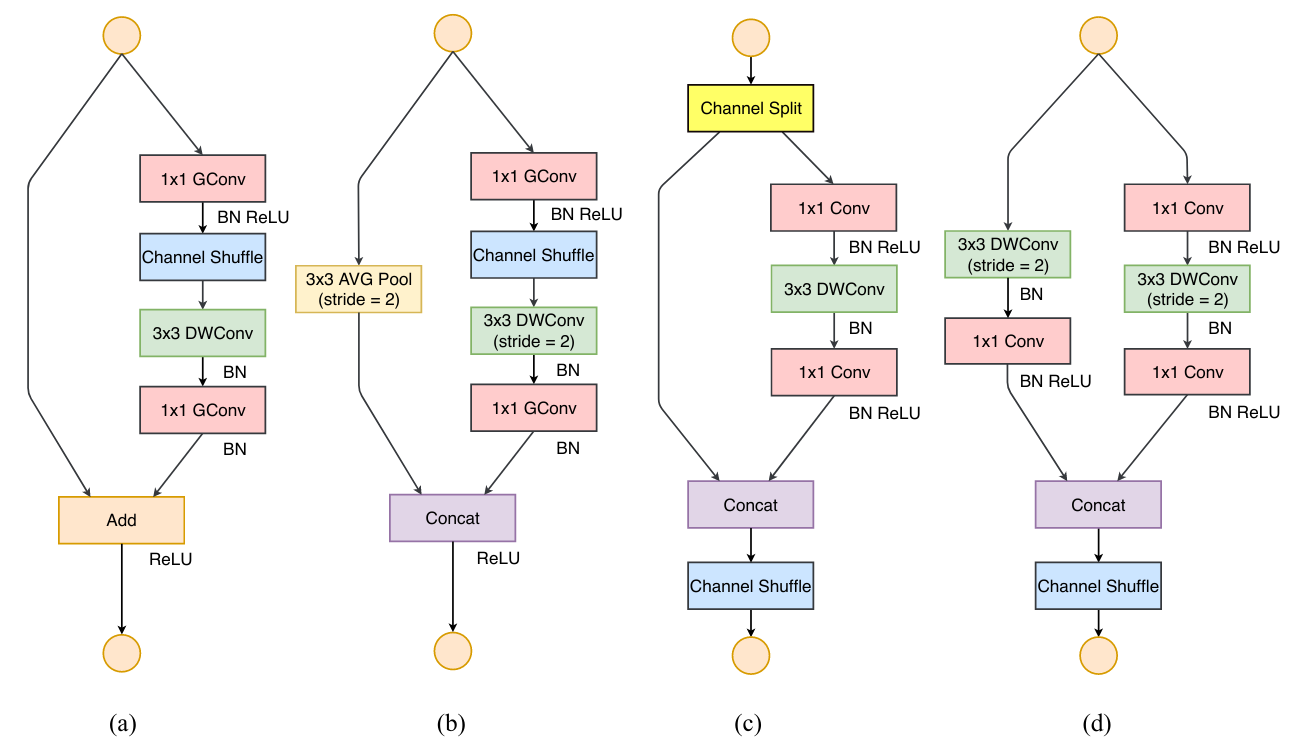
\includegraphics[width=1.0\textwidth]{images/shufflenetunits.png}}
	\caption[ShuffleNet and ShuffleNetV2 bottleneck units]{ShuffleNet (a), (b) and ShuffleNetV2 (c), (d) bottleneck units. (b) and (d) are units used for spatial downsampling with stride
	set to 2. (source \cite{bib:ma2018shufflenet})}
	\label{img:shufflenetunits}
\end{figure}

In the work of Ma et al. \cite{bib:ma2018shufflenet}, several practical guidelines
for efficient ConvNet architecture design have been raised. These are targeted mostly
to reduce MAC (memory access cost or the number of memory access operations).
Based on these guidelines, authors propose new architecture
called \textbf{ShuffleNetV2}. They replace group convolutions with pointwise $1\times 1$
convolutions and use channel split in downsampling unit. Otherwise, the number of stages and
units within them stays the same. Figure \ref{img:shufflenetunits} shows the difference between
ShuffleNet and ShuffleNetV2 units. Authors report their model is faster than MobileNetV2,
ShuffleNet and Xception. Moreover, with $\alpha=1$ it reaches $69.4\%$ top-1 accuracy.

ShuffleNetV2 has been studied further in order to employ it in semantic segmentation.
T{\"u}rkmen et al. \cite{bib:turkmen2019efficient} take ShuffleNetV2 as
an encoder and modify the last stage to omit downsampling and utilize dilated
convolution within depthwise-separable convolution. Decoding process is carried by
\textit{DeepLabV3+} \cite{bib:chen2018encoder} which contains
\textit{Dense Prediction Cell} \cite{bib:chen2018searching} at the beginning and
also makes use of dilated convolutions.
Authors report reaching $70.33\%$ mean IoU on Cityscapes dataset and $15.41$ FPS
on a mobile phone with an input image size of $224\times 224$.

\section{Active learning}
\label{sec:active_learning_rw}

Labeling a dataset for supervised learning is quite expensive and time consuming process.
\textit{Active learning} \cite{bib:settles2009active} 
is a technique where the model being trained participates in
the selection of its own training data. Selected samples are sent to the oracle (which
is a human expert in many cases) to annotate them and training continues on the enlarged
dataset. Training is stopped either when there are no more samples to annotate or the model
performs good enough and early stop condition is met. \cite{bib:sorsater2018}

There are several ways the model queries for new data. \textit{Pool-based} sampling is often used
in supervised learning. In theory, one sample is picked in each iteration and model is retrained.
However, during training ConvNet, querying one sample would be quite inefficient and
training would take
too much time. Therefore, querying batches is a common practice in the deep learning world.
\cite{bib:joshi2009multi, bib:vezhnevets2012active, bib:wang2016cost, bib:gal2017deep, bib:sener2017active, bib:yang2017suggestive, bib:mackowiak2018cereals, bib:zhdanov2019diverse}

\vspace{5mm}
Joshi et al. \cite{bib:joshi2009multi} propose active learning framework for training an
SVM classifier. They experiment with and compare random sampling, entropy based sampling
and margin sampling (called \textit{Best-versus-Second-Best} in their work) on three datasets.
Margin sampling showed up to be the best choice as they were able to reach higher accuracy with less
data.

The work of Vezhnevets et al. \cite{bib:vezhnevets2012active} discusses active learning in the
field of semantic segmentation. The authors try to bridge the gap between weakly supervised and fully
supervised methods by using active learning. The problem is modeled with a pairwise conditional random
field (CRF) defined over superpixels. Their active learning starts from the output
of weakly supervised learninng, meaning the labeling is partially incorrect. The model
is able to ask oracle about ground truth of specific superpixel.
They introduce a novel \textit{Expected Change} (EC) score. Instead of querying for most uncertain
images, they query for the ones that induce largest expected change in the labeling of the whole
training set in terms of upper-bound accuracy.
The disadvantage of this approach is that computing EC score is slow.
On the other hand, their algorithm beats standard entropy sampling and reaches $97\%$ of total
pixel accuracy of the corresponding fully supervised model while querying
less than 17\% of the superpixel labels.

Wang et al. \cite{bib:wang2016cost} study active learning and propose so called
\textit{Cost-Effective} active learning framework. Training the model starts with small amount
of unlabeled data. The models queries images to be annotated according to one of least confidence,
margin sampling or entropy. Moreover, unlabeled images the model is very confident on are
given \textit{pseudo-labels} and are added to training set with no human labor cost. At the end
of iteration, these pseudo-labeled images are returned to the pool of unlabeled ones.
Authors state that their algorithm performs better than random selection. However, the analysis in
\cite{bib:sener2017active} shows it actually performs worse than random sampling.

Several acquisition function are studied by Gal et al. \cite{bib:gal2017deep} in their
Bayesian ConvNet setting recognizing hand-written digits from MNIST dataset.
These function are max entropy, BALD, variation ratios, mean STD and random baseline. Both
mean STD and random sampling under-perform compared to the other functions.

Another work is presented by Sener et al. \cite{bib:sener2017active}. Their sampling strategy
is based on \textit{k-center} algorithm which strives for finding $k$ points which minimize
distance from all points to their closest core point. The authors demonstrate that random sampling
is in many cases much more effective than uncertainty methods. This is because images the model
is most uncertain on are often similar and thus do not cover the sample space appropriately.
They evaluate models on several datasets achieving state-of-the-art results.

Active learning for biomedical image segmentation has also been successfully used by
Yang et al. \cite{bib:yang2017suggestive}. Image sampling is based on the uncertainty information
as well as similarity information. Last layer in the encoding part produces high level feature
embedding which is then used for computing cosine distance between images. Their approach
achieves state-of-the-art performance by using only $50\%$ of the training data.

It seems that awareness of image diversity is one of the most important criterion. Images may
be embedded into vector space and clustered by K-means algorithm as stated in 
\cite{bib:zhdanov2019diverse}.

\section{Previous approaches with Smelý Zajko}
\label{sec:prev_approaches}

The robot \textit{Smelý Zajko} (\textit{Brave Rabbit} in English), shown in Figure \ref{img:zajko},
began its journey to discover and drive through city parks in 2011.
The work of M. Nadhajský \cite{bib:nadhajsky2011} aims to propose a design
of the outdoor robot for this kind of competition.
This design includes construction from aluminium and wooden parts
as well as different hardware parts like servo motors, sensors and wheels. The author
also implements algorithms for controlling the robot and verifies its functionality
in the outdoor environment. The proposed solution for dealing with recognition of
driveable path makes use of multi-layer perceptron (MLP).

M. Moravčík continued on robot's improvements in his thesis \cite{bib:moravcik2013}.
The author focuses on improving robot's localization and planning based on Open Street Maps.
Moreover, the author introduces vision module for predicting driveable path which utilizes
MLP and various preprocessing methods. Camera's image is first being
converted into CIELAB color space and then cut into smaller patches of size $5\times 5$.
The author also tests various MLP architectures as well as other handcrafted
features such as histograms, regions with high driveable probability etc.

The work of J. Dúc \cite{bib:duc2017} describes integration of a new laser sensor and
based on the analysis of the previous state of the robot, he decides to change the system
architecture
and rewrite the software into \textit{Robot Operating System} (ROS) \cite{bib:quigley2009ros}.
ROS aims to be modular with the ability to divide subsystems into modules which are able 
to communicate between each other and are portable when it comes to integrating them
to other system. It also supports recording and logging data from sensors and replaying 
them afterwards. The author also designs new reactive algorithm for detecting and avoiding
obstacles and tests it in both indoor and outdoor environment.

Jariabka et al. \cite{bib:suppajariabka2017} extended previous MLP approaches in
aforementioned works. They evaluate baseline MLP models on their dataset with images
of size $224\times 224$ pixels and propose the first ConvNet model used on
\textit{Smelý Zajko}. Its architecture is rather simple having several convolutional layers
with 10 filters followed by ReLU nonlinearity and max-pooling $2\times 2$ layers. Authors
also experiment with deeper architecture containing fully-connected layer and two
convolutional blocks.

The solution used at RoboTour 2018 is based on HSV data extracted from training images.
Every image is converted into HSV color space and processed pixel by pixel. Only
\textbf{H} and \textbf{S} components are taken into account. The model creates 2D
matrix with values expressing how likely is the pixel with specific H and S driveable.

\begin{figure}[!h]
	\centerline{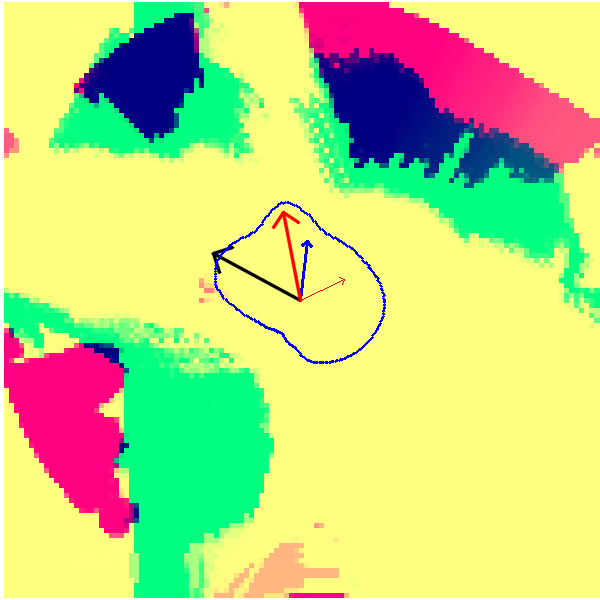
\includegraphics[width=0.45\textwidth]{images/localmap.png}}
	\caption[Example of Local Map at the crossroad]{Example of Local Map at the crossroad.
	Robot is deciding which exit to use. The yellow color denotes driveable trail and blue or red are obstacles calculated by laser sensor.}
	\label{img:localmap}
\end{figure}

In 2019, M. Fikar \cite{bib:fikar2019} continued on improving robot's algorithm for planning and
localization. The robot reads data from sensors, tries to combine them and creates so called
\textit{Local Map}. Based on this data, the robot calculates the best direction towards
destination point and sends the information about next move to motor control unit, which is in
our case Arduino. The map also takes predicted driveable path into account.
An example of this map is presented in Figure \ref{img:localmap}.

\vspace{5mm}
All of the aforementioned models for predicting driveable path
are looking at specific regions discarding spatial information which makes them
less precise. This causes the models to make mistakes in classifying shadows, segments
with color similar to the road and images with varying lighting conditions.
To deal with such a problem we will focus on incorporating a ConvNet taking whole image as
input and outputting dense pixel-wise segmentation mask.